\section[Основные положения теории искусственных нейронных сетей]{%
  ОСНОВНЫЕ ПОЛОЖЕНИЯ ТЕОРИИ \\
  ИСКУССТВЕННЫХ НЕЙРОННЫХ СЕТЕЙ
}

\subsection{Искусственный нейрон}

Под \emph{нейронными сетями} подразумеваются вычислительные структуры,
которые моделируют простые биологические процессы,
обычно ассоциируемые с процессами человеческого мозга.
Элементарным преобразователем в данных сетях является \emph{искусственный нейрон}
или просто нейрон, названный так по аналогии с биологическим прототипом~\cite{kruglov2001}.

На рисунке~\ref{fig:struct_neuron} показана структура искусственного нейрона.
В соответствии с ней, в состав нейрона входят умножители (синапсы),
сумматор и нелинейный преобразователь.

\begin{figure}[h!]
  \centering
  \fcolorbox{gray}{white}{
    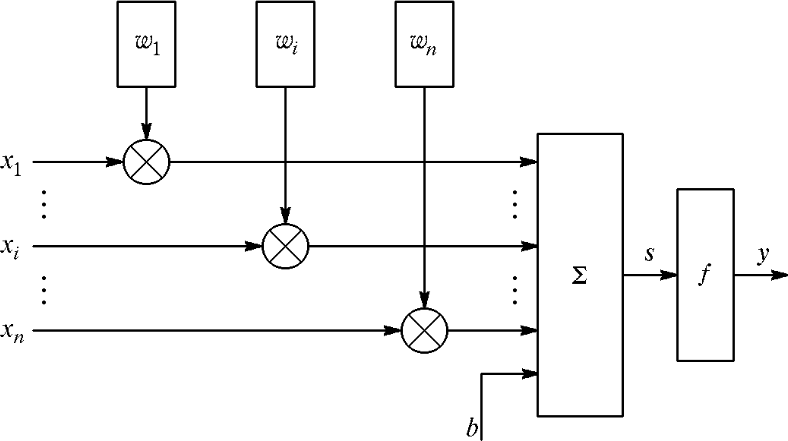
\includegraphics[width=120mm]{fig/struct_neuron}
  }
  \caption{Структура искусственного нейрона}
  \label{fig:struct_neuron}
\end{figure}

\emph{Синапсы} осуществляют связь между нейронами и умножают входной сигнал на число,
характеризующее силу связи, --- вес синапса.
\emph{Сумматор} выпроняет сложение сигналов, поступающих по синаптическим связям от
других нейронов и внешних входных сигналов.
\emph{Нелинейный преобразователь} реализует нелинейную функцию одного аргумента,
называемую \emph{функцией активации}.
Одной из наиболее распространенных функций активации является
так называемая \emph{логистическая функция}, или сигмоид
\[
  f(s) = \dfrac{1}{1 + e^{-as}}.
\]

\subsection{Обучение нейронной сети}

Искусственные нейроны, объединяясь между собой, образуют нейронную сеть,
которая выполняет поставленную перед ней задачу.
В процессе функционирования нейросети можно выделить два этапа:
\begin{enumerate}
\item Обучение, в ходе которого производится настройка сети на основании
  учебных примеров исходных данных, носящих репрезентативный характер.
\item Применение, в ходе которого осуществляется решение
  поставленной задачи классификации, прогнозирования, управления и~т.~п.
  на основании реальных исходных данных.
\end{enumerate}

В ходе обучения сети с учителем на основании сопоставления
результата её работы с эталоном выполняется оптимизация её параметров.
Одним из наиболее известных методов корректирования параметров нейронной сети
является \emph{метод обратного распространения ошибки}.
Приведем его словесное описание.
\begin{enumerate}
\item Весам сети присваиваются некоторые начальные значения.
\item Выбирается очередная обучающая пара \( (\mathbf{X}, \mathbf{Y}) \)
  из обучающего множества; вектор \( \mathbf{X} \) подается на вход сети.
\item Вычисляется выход сети \( \mathbf{Y}_0 \).
\item Вычисляется разность между требуемым (целевым, \( \mathbf{Y} \))
  и реальным (вычисленным, \( \mathbf{Y}_0 \)) выходом сети.
\item Параметры сети \( w_i \) корректируются так, чтобы минимизировать ошибку.
\item Шаги 2--5 повторяются для каждой пары обучающего множества до тех пор,
  пока ошибка на всем множестве не достигнет приемлемой величины.
\end{enumerate}

\subsection{Гибридные сети}

Теоретически, системы с нечеткой логикой и искусственные нейросети эквивалентны
друг другу, однако на практике у них имеются свои собственные достоинства и недостатки.
Например, нейронные сети хороши для задач распознавания образов, но весьма неудобны
для выяснения вопроса, как они подобное распознавание осуществляют.
Они могут приобретать знания, но процесс их обучения зачастую происходит достаточно
медленно, а анализ обученной информации весьма сложен.
При этом ввести в нейронную сеть какую-либо априорную информацию для ускорения
её обучения невозможно.
Системы с нечеткой логикой, напротив, хороши для объяснения получаемых с их
помощью выводов, но они не могут автоматически приобретать знания для использования
их в механизмах выводов.
Подобные соображения легли в основу аппарата гибридных сетей,
способных не только использовать априорную информацию,
но и приобретать новые знания, оставаясь при этом логически прозрачными для пользователя.

\emph{Гибридная нейронная сеть} --- это нейронная сеть с четкими сигналами,
весами и активационной функцией, использующая для объединения сигналов
t-норму, t-конорму или некоторые подобные им функции.

Рассмотрим примеры элементарных гибридных сетей.
\begin{enumerate}
\item Нечеткий нейрон <<И>>.
  В данном случае сигналы \( x_i \) и веса \( w_i \) объединяются с помощью t-конормы:
  \( p_i = S(w_i, x_i), \: i = 1, 2, \)
  а выход образуется с применением t-нормы:
  \( y = T(p_1, p_2) = T(S(w_1, x_1), S(w_2, x_2)), \)
  как показано на рисунке~\ref{fig:hybrid_and}.

  \begin{figure}[h!]
    \centering
    \fcolorbox{gray}{white}{
      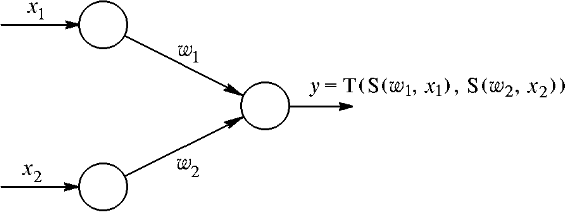
\includegraphics[width=92mm]{fig/hybrid_and}
    }
    \caption{Структура гибридного нейрона <<И>>}
    \label{fig:hybrid_and}
  \end{figure}

\item Нечеткий нейрон <<ИЛИ>>.
  В данном случае сигналы \( x_i \) и веса \( w_i \) объединяются с помощью t-нормы:
  \( p_i = T(w_i, x_i), \: i = 1, 2, \)
  а выход образуется с применением t-нормы:
  \( y = S(p_1, p_2) = S(T(w_1, x_1), T(w_2, x_2)), \)
  как показано на рисунке~\ref{fig:hybrid_or}.

  \begin{figure}[h!]
    \centering
    \fcolorbox{gray}{white}{
      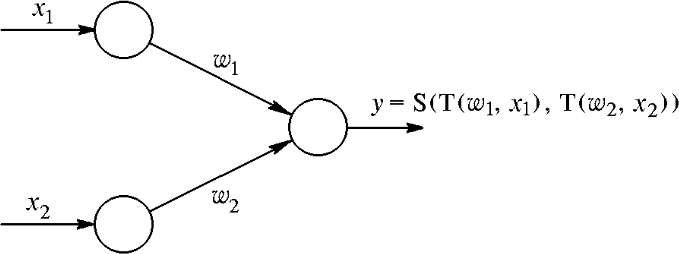
\includegraphics[width=92mm]{fig/hybrid_or}
    }
    \caption{Структура гибридного нейрона <<ИЛИ>>}
    \label{fig:hybrid_or}
  \end{figure}
\end{enumerate}
